\chapter{Enabling Structured Illumination Microscopy at greater depth}

\section{Sample Induced Aberrations in Structured Illumination Microscopy}
\label{sec:sample_aberrations_SIM}

The origin of optical aberrations and their effect on image
formation from a geometric optics standpoint and how this leads 
decreased image quality and resolution has already been covered 
in Section~\ref{sec:aberrations}. The extent of optical 
aberrations in thick samples and the particular effects of
aberrations on structured illumination microscopy (SIM) imaging 
are worth paying particular attention to. 

In widefield microscopy, an even field of illumination is 
applied to the field of view and the resultant fluorescent
signal from the sample is measured. In SIM, this even 
illumination is replaced by a sinusoidally varying
illumination pattern. Multiple images with varying angle 
and phase shifts to the illumination pattern are acquired. 
These images are then used to reconstruct a single 
super-resolved image\cite{gustafsson2000surpassing,gustafsson2008three}.
Recall a single fluorescent image, $F(\textbf{r})$, is 
defined by:

\begin{equation}
\begin{split}
F(\textbf{r}) &= (E \circledast H)(\textbf{r})\\
F(\textbf{r}) &= [D(\textbf{r})I(\textbf{r})] \circledast H(\textbf{r}),\\
\end{split}\tag{\ref{eq:fluorescent_image}}
\end{equation}

Where $D(\textbf{r})$ is the sample fluorescence distribution, 
$I(\textbf{r})$ is the illumination pattern, $E(\bar{x})$ is
the resultant emission signal and $H(\textbf{r})$ is the system 
point spread function (PSF). Section~\ref{sec:aberrations} has already
discussed the effect aberrations have on distorting the system
PSF, $H(\textbf{r})$. However, in SIM imaging the illumination 
pattern, $I(\textbf{r})$, is also formed in the same imaging path
and is therefore the illumination pattern formation is also 
affected by the system aberrations.

Consider the illumination pattern function. Fully coherent
illumination conditions yield optimum imaging performance and
are therefore chosen. In practice, only partially coherent 
conditions are achievable. Utilising the fully coherent 
approximation, $I(\textbf{r})$ can be expressed as:

\begin{equation}\label{eq:SIM_illumination}
I(\textbf{r}) = \left\| \frac{1}{2}[1 + \cos(\textbf{r}\bullet\textbf{p} + \phi)]\circledast H_{amp}(\textbf{r}) \right\|^{2}
\end{equation}

Where $\textbf{p}$ and $\phi$ define the orientation and phase of
the illumination pattern respectively. $H_{amp}(\textbf{r})$ is the
amplitude PSF, as opposed to $H(\textbf{r})$ which is the intensity
PSF and is defined as:

\begin{equation}\label{eq:amplitude_PSF}
H_{amp}(\textbf{r}) = \mathcal{F}[P(\textbf{r}')]
\end{equation}

Where $P$ is the pupil function, $\textbf{r}'$ is the coordinate
vector in the pupil plane and $\mathcal{F}$ is the Fourier
transform operation. Utilizing the Fourier convolution 
theorem, Equation~\ref{eq:SIM_illumination} becomes:

\begin{equation}\label{eq:SIM_illumination_invFT}
I(\textbf{r}) = \left\| \mathcal{F}^{-1}\left\{\frac{1}{2}\left[\delta(\textbf{r}') + \frac{\exp^{-i\theta}}{2}\delta(\textbf{r}'-\textbf{p}) + \frac{\exp^{i\theta}}{2}\delta(\textbf{r}'+\textbf{p})\right]P(\textbf{r}')\right\} \right\|^{2}
\end{equation}

Where value of $\textbf{p}$ positions the delta functions in the
pupil plane. $\textbf{p}$ is chosen to have a value of or close
to 1, to maximise the resolution increase. 
Equation~\ref{eq:SIM_illumination_invFT} there is clearly only
illumination at three points in the pupil plane, at the centre 
and diametrically opposed at the edge of the pupil. There are
two principle consequences of this fact. Firstly, since the 
illumination only exists at the centre and edges of the pupil
plane, the illumination pattern is only affected by phase 
variations at those points. Therefore, the illumination pattern
should be immune to aberrations with little phase variation at 
the edges of the pupil. Secondly, rotationally symmetrical 
aberrations, such as spherical aberration, have the main
effect of refocusing the illumination pattern\cite{booth2015aberrations}.

It has also been shown that the imaging properties of a SIM
system and the quality of the reconstructed super-resolution
images are determined by the system's ability to reliably
image the high spatial frequencies\cite{debarre2008adaptive,thomas2015enhanced}.
The aberrations which affect the strength of high spatial 
frequency signals can be divided into two categories; 
isoplanar and anisoplanar aberrations. Single adaptive 
elements, such as the deformable mirror in the DeepSIM 
setup, can only correct for the isoplanar aberrations.
Anisoplanar aberrations will still introduce artifacts 
in the final, reconstructed data. However, provided that
the anisoplanar aberrations are considerably smaller than
the isoplanar aberrations, these aberrations will be small
compared to the SIM image and will not prevent a successful
reconstruction\cite{thomas2015enhanced}.

The cumulative effect of the optical aberrations is that
traditional SIM imaging is limited in its imaging depth to
approximately $10-20\mu m$\cite{schermelleh2019super,wu2018faster}. However, 
correcting the optical aberrations present would not yield
an infinite depth of imaging due to scattering of photons,
which increases with depth. Nonetheless, by correcting for
optical aberrations present DeepSIM offers the potential to 
acquire super-resolution SIM images at an unprecedented depth.

\section{IsoSense}
\label{sec:isosense}

Anisotropies in the sample fluorescence distribution can bias 
the corrections towards improving the image quality in a 
non-uniform manner. There has recently been a technique developed 
to overcome  this issue; IsoSense\cite{vzurauskas2019isosense}. 
It relies  on producing spatially structured light in order to fill 
empty sections of the image Fourier spectrum. IsoSense is designed 
to be used in structured illumination microscopy (SIM) setups since 
they often incorporate spatial light modulators (SLM) as high-speed, 
dynamic diffraction  gratings and SIM is particularly sensitive to 
Fourier space anisotropies.

Microscope-AOtools incorporates the methods necessary to implement
IsoSense. Figure~\ref{fig:isosense_visualisation} shows both
the structured illumination pattern applied to the SLM 
and the location of the beams in Fourier space. The illumination
pattern shown in Figure~\ref{fig:isosense_visualisation_real} is
the inverse Fourier transform of the 4-beam interference pattern 
in Figure~\ref{fig:isosense_visualisation_ft}. The location 
of these beams, $\kappa$, are: 
$(0,0)$, $(0,\gamma \omega_{l})$, $(0,-\gamma \omega_{l})$, 
$(\gamma \omega_{l}, 0)$, $(-\gamma \omega_{l}, 0)$, 
$(\frac{\gamma \omega_{l}}{2}, \frac{\gamma \omega_{l}}{2})$, 
$(-\frac{\gamma \omega_{l}}{2}, \frac{\gamma \omega_{l}}{2})$, 
$(\frac{\gamma \omega_{l}}{2}, -\frac{\gamma \omega_{l}}{2})$, 
$(-\frac{\gamma \omega_{l}}{2}, -\frac{\gamma \omega_{l}}{2})$. 
$u,v$ are the spatial frequency analogues of the $x,y$ axes. 
$\omega_{l}$ is the lateral diffraction limit in reciprocal space 
as per Equation~\ref{eq:lateral_spatial_freq_res} and $\gamma$ is 
a user defined fill fraction. This fill fraction controls the 
positions of the beams in the interference pattern and hence the 
region of the Fourier spectrum which will be enhanced over normal 
illumination. The resultant emission image  obtained, $E(\textbf{r})$, 
can be described as:

\begin{equation}\label{eq:isosense_real}
E(\textbf{r}) = D(\textbf{r}) \times I(\textbf{r})
\end{equation}	

Where $I(\textbf{r})$ is the interference pattern, similar to that shown in 
Figure\ref{fig:isosense_visualisation_real}, $D(\textbf{r})$ is the sample 
fluorescence distribution as before and $\textbf{r}$ is the spatial 
coordinate vector. Applying a Fourier transform yields:

\begin{equation}\label{eq:isosense_ft}
\begin{split}
\mathcal{F}[F(\textbf{r})] &= \mathcal{F}[D(\textbf{r})\times I(\textbf{r})] \\
\tilde{\textbf{F}}(\textbf{k}) &= \tilde{\textbf{D}}(\textbf{k}) \circledast \tilde{\textbf{I}}(\textbf{k}) \\
\tilde{\textbf{F}}(\textbf{k}) &= \sum_{\kappa}\iint\tilde{\textbf{D}}(\textbf{k})\delta(\textbf{k} - \kappa)dudv \\
\tilde{\textbf{F}}(\textbf{k}) &= \sum_{\kappa}\tilde{\textbf{D}}(\textbf{k} - \kappa)
\end{split}
\end{equation}

Where $\tilde{\textbf{F}}(\textbf{k})$, $\tilde{\textbf{I}}(\textbf{k})$ and 
$\tilde{\textbf{D}}(\textbf{k})$ are the Fourier transforms of $F(\textbf{k})$, 
$I(\textbf{k})$ and $D(\textbf{k})$, the $\kappa$ frequencies are the 
locations of interference pattern beams described above and $\textbf{k}$ is 
the spatial frequency vector. By convolving the sample fluorescence 
distribution with  multiple $\delta$-functions, multiple copies of the 
sample spatial frequency information are created and regions of the 
system OTF left  unfilled by sample fluorescence distribution anisotropies 
are filled, leading to  improved sampling of the system OTF particularly 
at high spatial frequencies close to $w$ and greater aberration 
sensitivity\cite{vzurauskas2019isosense}.

\begin{figure}[h]
	\centering
	\begin{subfigure}{0.4\textwidth}
		\centering
		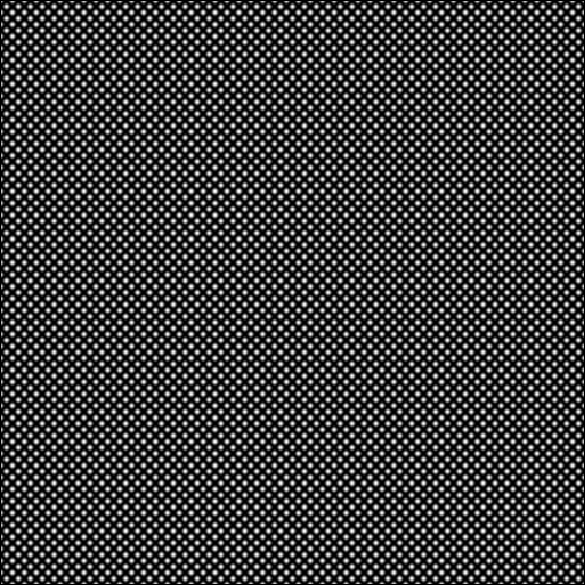
\includegraphics[width=1\linewidth, scale=0.5]{./images/isosense_visualisation_real.png}
		\caption{}
		\label{fig:isosense_visualisation_real}
	\end{subfigure}
	\begin{subfigure}{0.4\textwidth}
		\centering
		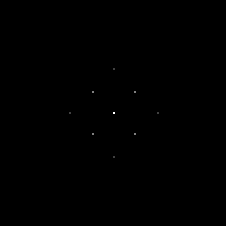
\includegraphics[width=1\linewidth, scale=0.5]{./images/isosense_visualisation_ft.png}
		\caption{}
		\label{fig:isosense_visualisation_ft}
	\end{subfigure}
	\caption[IsoSense pattern visualisation.]{IsoSense pattern visualisation. \textbf{(a)} A simulated IsoSense pattern created with a 4-beam interference. A pattern similar to this is applied to the SLM \textbf{(b)} A diagram of a 4-beam interference pattern in Fourier space. The diagonal axis and the horizontal/vertical axis have $\frac{1}{2}$ and $\frac{1}{4}$ of the intensity of the central beam respectively.}
	\label{fig:isosense_visualisation}
\end{figure}

\section{Biological Exemplar}
\label{sec:DeepSIM_biology}

To demonstrate the improvement in image quality adaptive optics
provides in the DeepSIM system, we utilise the 
\textit{Drosophila melanogaster} neuro-muscular junction (NMJ) sample.

\subsection{Sample preparation}
\label{subsec:DeepSIM_sample_prep}

The samples were prepared by following the 
protocol\cite{brent2009drosophila}. 3rd instar \textit{Drosophila 
	melanogaster} larvae (Bruchpilot (Brp)-GFP strain) were dissected in HL3 
buffer with 0.3mM $\text{Ca}^{2+}$ to prepare a so-called larval fillet,
and the larval brains were removed. After this, larvae were stained for 15 
minutes with Horseradish Peroxidase (HRP) conjugated to Alexa568 
fluorophore to visualise the neurons, washed with HL3 buffer with 0.3mM 
$\text{Ca}^{2+}$ and imaged in HL3 buffer with 0mM $\text{Ca}^{2+}$ to 
prevent the larvae from moving.

\section{Experimental Results}
\label{sec:DeepSIM_results}

\subsection{Experimental Setup}
\label{subsec:DeepSIM_setup}

As previously notes, the theoretical resolution extension factor for 
a diffraction limited SIM system is given by:

\begin{equation}
\alpha_{l} = \frac{\left(\frac{1}{\lambda_{ex}} + \frac{1}{\lambda_{em}}\right)}{\frac{1}{\lambda_{em}}} = 1 + \frac{\lambda_{em}}{\lambda_{ex}}.\tag{\ref{eq:lateral_res_extension_factor}}
\end{equation}

There are two complicating factors. Firstly, as mentioned in 
Section~\ref{subsec:fluorescence}, fluorescent proteins do not present 
a single wavelength of emission, $\lambda_{em}$ but rather have an 
emission spectrum. For simplicity, the peak of the emission spectrum is
used to calculate the resolution extension. Secondly, 
Equation~\ref{eq:lateral_res_extension_factor} assumed that the locations
of the $m=\pm2$ Fourier components of the illumination pattern are placed
at $\left|\textbf{k}\right| = \frac{1}{\lambda_{ex}}$. This is not 
necessarily the case. As such, an accurate measure of the theoretical
resolution extension factor for a practical SIM implementation is given as:

\begin{equation}\label{eq:lateral_res_extension_factor_real}
\alpha_{l} = \frac{\left(\frac{1}{\lambda_{I}} + \frac{1}{\lambda'_{em}}\right)}{\frac{1}{\lambda'_{em}}} = 1 + \frac{\lambda'_{em}}{\lambda_{I}},
\end{equation}

where $\lambda'_{em}$is the wavelength of the peak of the emission 
spectrum and $\lambda_{I}$ is the stripe width of the illumination
pattern. For DeepSIM, the conventional resolution limit for the 
green and red channels respectively is $291$nm and $338$nm. The stripe 
width was $322$nm and $367$nm for $488$nm and $561$nm excitation
wavelengths respectively.

To verify both that the system is capable of achieving super-resolution
and that Microscope-AOtools is capable of correcting for optical 
aberrations, the Argolight SIM slide was image. The structure chosen for
imaging was a set of pairs of $36 \mu$m-long horizontal lines pairs lines 
which spacing gradually increases, from $0$ to $390$nm, with a step of 
$30$nm. 

This structure was chosen for two principle reasons. Firstly, the known
separation of the fluorescent structures allows for an accurate gauge of 
the system resolving power. The structure was excited at $488$nm and 
measured with a peak emission wavelength of $610$nm. Therefore, utilising 
Equation~\ref{eq:lateral_res_extension_factor_real} the diffraction 
limited lateral resolution in a SIM reconstruction would be $161$nm i.e. 
the first 6 separations should not be resolvable. Secondly, the refractive 
index of the Argolight slide at $488$nm is 1.53 and the structures are 
positioned at $170\mu$m below the top glass surface\cite{argolight2017user}.
This represents a significant source of optical aberrations, primarily
spherical aberration, which would degrade the image quality and decrease
resolution in the absence of AO correction.

Figure~\ref{fig:Argolight_slide_both} shows both the maximum intensity 
projection of $13\mu$m SIM z-stacks and a $xz$ slice at the midpoint of 
the $y$-axis. In both datasets, the $150$nm separation is resolvable, which 
is slightly better than the anticipated lateral resolution. This is not 
entirely surprising as the Argolight sample is a highly fluorescent, 
regular structure with very little out-of-focus fluorescence to compromise 
the image quality. As mentioned in Section~\ref{subsec:resolution}, the 
assumptions used to estimate the lateral resolution leave a number of 
factors unaccounted for and mainly provide a useful 
estimate\cite{den1997resolution}. For a structure such as that present 
in the Argolight slide, a slight over-performance is normal. There are 
significant artifacts present in the dataset without AO correction which 
makes separations $+150$nm unresolvable in parts. The $z$ length of the 
structures in the $xz$ slice is also extended and shows significant 
artifacts, primarily ``echo'' structures above the true fluorescent 
structures. Additionally, the dataset without AO correction has half the 
intensity of the dataset with AO correction and must be displayed on a 
reduced dynamic range for visibility. Applying the AO correction recovers 
the fluorescent signal and removes these artifacts. The spherical 
aberration mismatch measurements obtained from the ImageJ plugin SIMCheck 
in Figures~\ref{fig:Argolight_spherical_mismatch_woAO} and 
\ref{fig:Argolight_spherical_mismatch_AO} confirms that the AO has 
successfully removed the majority of the spherical aberration 
present\cite{ball2015simcheck}.

\begin{figure}
	\centering
	\begin{subfigure}[t]{0.45\textwidth}
		\centering
		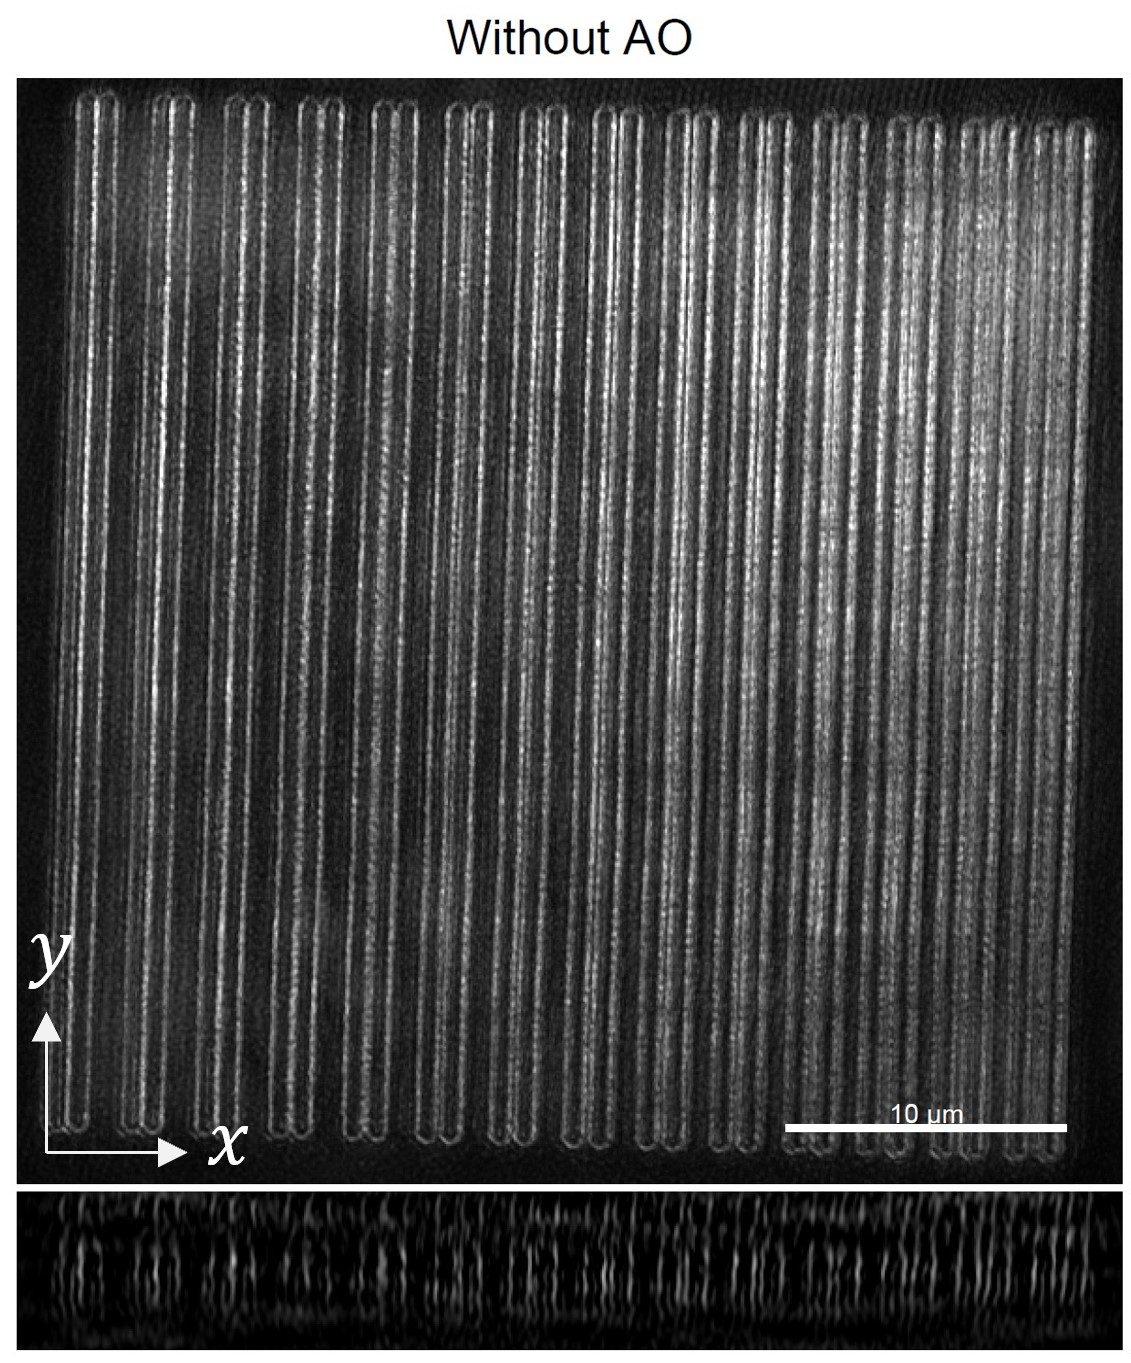
\includegraphics[width=\linewidth]{images/Argolight_slide_woAO_axis.jpg}
		\caption{}
		\label{fig:Argolight_slide_woAO_axis}
	\end{subfigure}
	\begin{subfigure}[t]{0.45\textwidth}
		\centering
		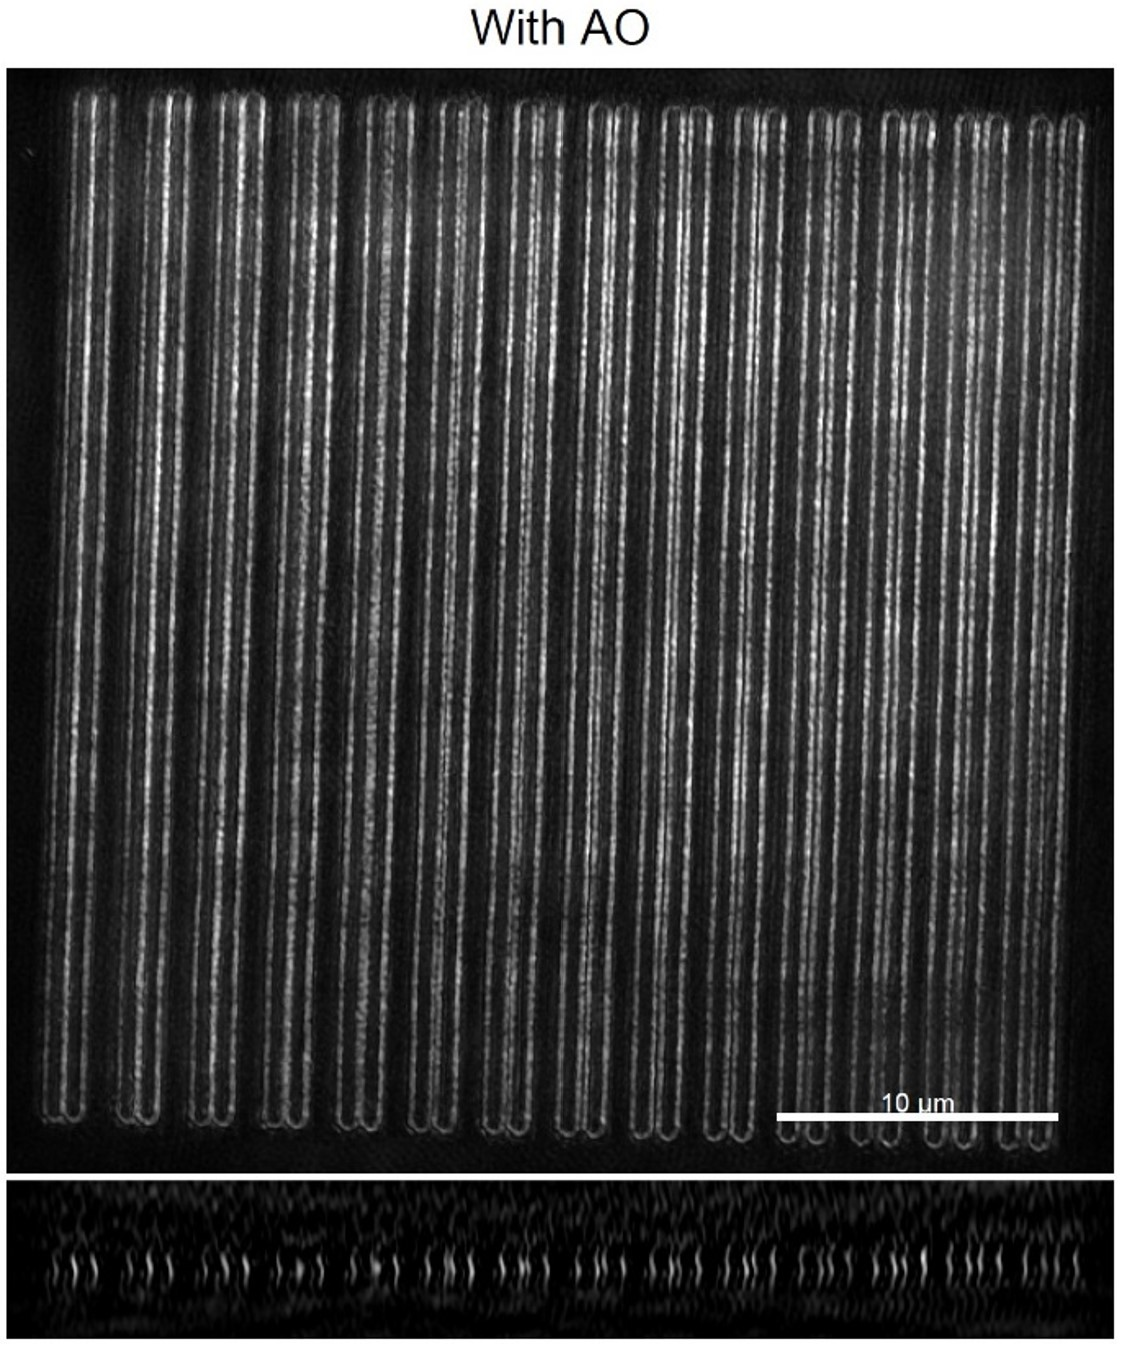
\includegraphics[width=\linewidth]{images/Argolight_slide_AO.jpg}
		\caption{}
		\label{fig:Argolight_slide_AO}
	\end{subfigure}
	
	
	\begin{subfigure}[t]{0.45\textwidth}
		\centering
		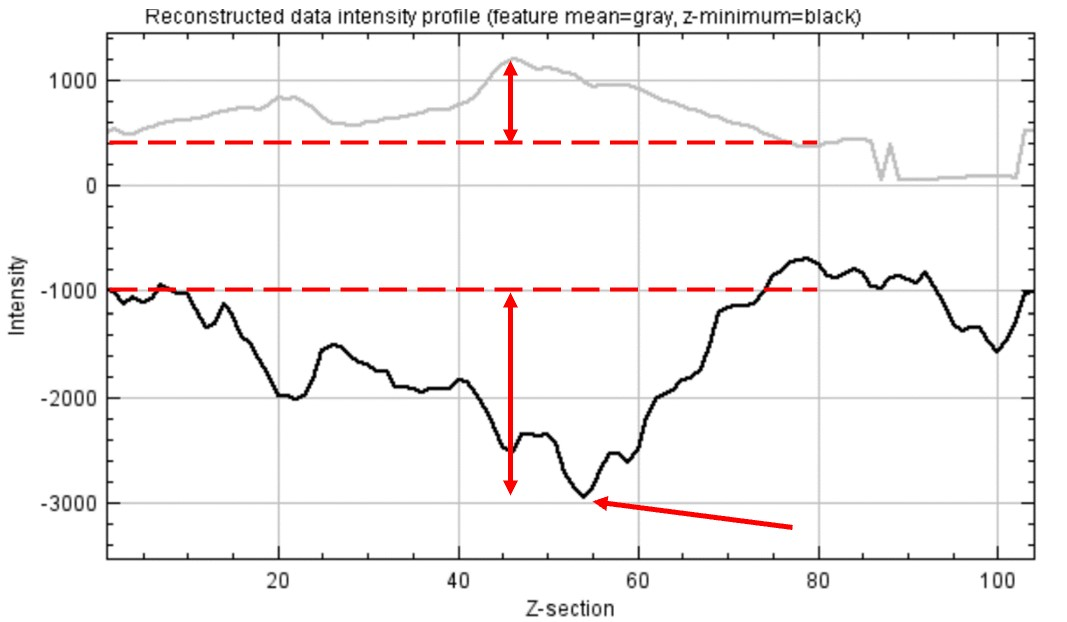
\includegraphics[width=\linewidth]{images/Argolight_spherical_mismatch_woAO.jpg}
		\caption{}
		\label{fig:Argolight_spherical_mismatch_woAO}
	\end{subfigure}
	\begin{subfigure}[t]{0.45\textwidth}
		\centering
		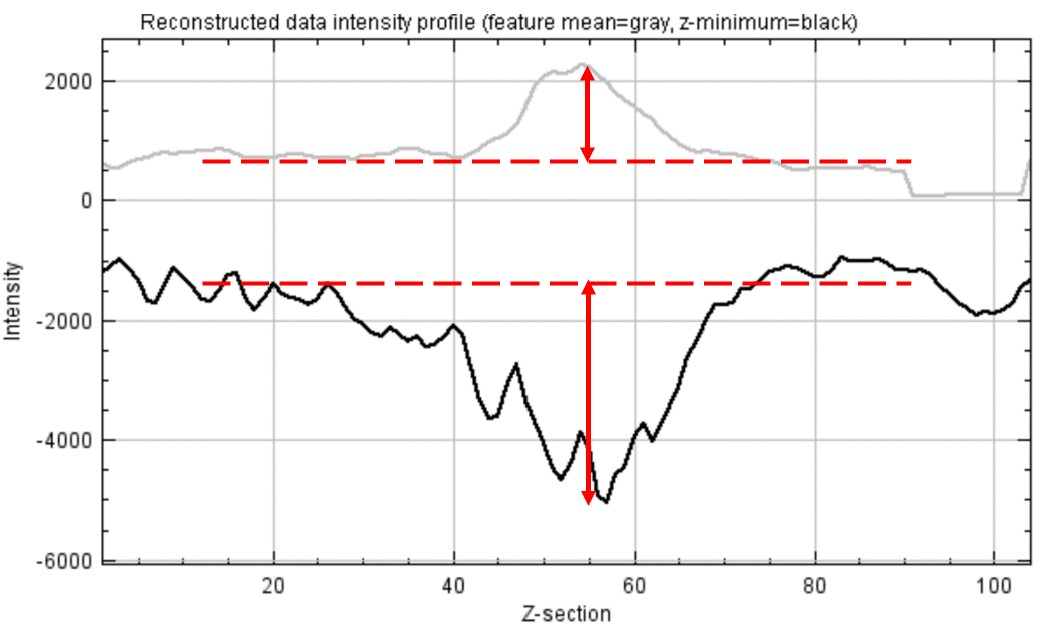
\includegraphics[width=\linewidth]{images/Argolight_spherical_mismatch_AO.jpg}
		\caption{}
		\label{fig:Argolight_spherical_mismatch_AO}
	\end{subfigure}
	\caption[Argolight slide data]{Argolight slide data. Both \textbf{(a)} without AO correction and \textbf{(b)} with AO correction datasets 
		are maximum intensity projection of $13\mu$m SIM z-stacks (top) and 
		a $xz$ slice at the midpoint of the $y$-axis (bottom). Without AO correction data is displayed with the maximum intensity level of data with AO correction for clarity. The spherical aberration mismatch from the SIMCheck ImageJ plug-in\cite{ball2015simcheck} is shown \textbf{(c)} without AO correction and \textbf{(d)} with AO correction}
	\label{fig:Argolight_slide_both}
\end{figure}

For the NMJ data obtained, the sensorless correction routine detailed in 
Section~\ref{subsec:sensorless_correction} using the Fourier Power image 
quality metric described in Section~\ref{subsec:fourier_power_metric} since 
it is well suited to maximising the spatial frequency content essential to
SIM imaging. The aberrations corrected were: primary and secondary 
spherical, oblique and vertical astigmatism, vertical and horizontal coma, 
and oblique and vertical trefoil - corresponding to Noll indices 11, 22, 5, 
6, 7, 8, 9, and 10. These modes were corrected in the order they are listed
here. They were corrected with the IsoSense pattern applied to the SLM. The 
range of amplitudes applied was [-1.5 radians, 1.5 radians] over 9 images, 
with 2 iterations for a total of 144 images for a complete correction 
routine. These variables were specified in the dialogue box shown in 
Figure~\ref{fig:DM_sensorless_ao_parameters}.

Figure~\ref{fig:DeepSIM_NMJ_data} shows maximum intensity projections of 12.75$\mu$m $z$-stacks obtained with the centre of the stack $\sim20\mu$m deep in the sample, both without and with aberration correction. Despite the sensorless adaptive optics routine being performed only using the data 
from the Alexa568 (HRP) channel, improvements in intensity and contrast
are observed in both imaging channels. Much of the membrane labelled-HRP is 
not visible without AO correction. Almost all of the BRP is extremely dim 
or invisible without AO correction. The insets in 
Figures~\ref{fig:DeepSIM_NMJ_woAO_ROI1_GFP} -
\ref{fig:DeepSIM_NMJ_AO_ROI2_Alexa568} show subsections of the dataset 
where structures which are invisible or of poor contrast without AO 
correction become visible.

\begin{figure*}
	\centering
	\begin{subfigure}[t]{0.49\textwidth}
		\centering
		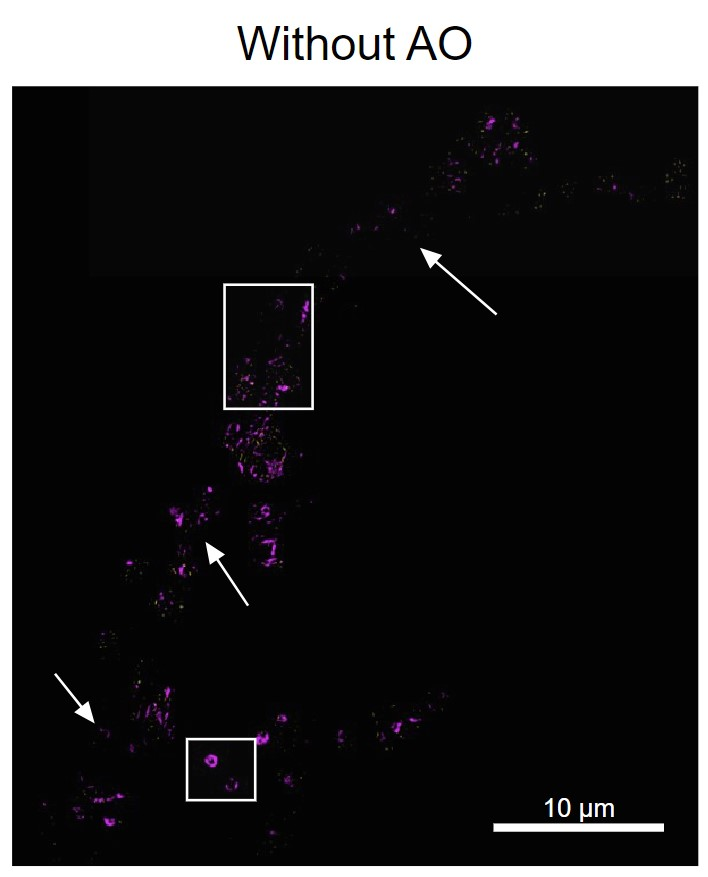
\includegraphics[width=\linewidth]{images/DeepSIM_NMJ_woAO.jpg}
		\caption{}
		\label{fig:DeepSIM_NMJ_woAO}
	\end{subfigure}
	\begin{subfigure}[t]{0.49\textwidth}
		\centering
		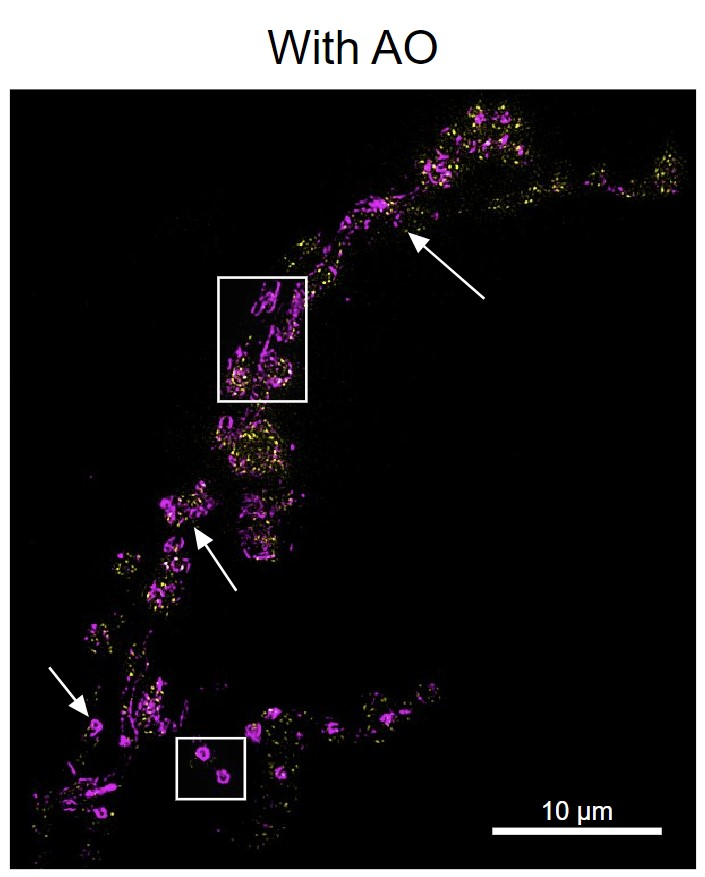
\includegraphics[width=\linewidth]{images/DeepSIM_NMJ_AO.jpg}
		\caption{}
		\label{fig:DeepSIM_NMJ_AO}
	\end{subfigure}
	
	
	\begin{subfigure}[t]{0.237\textwidth}
		\centering
		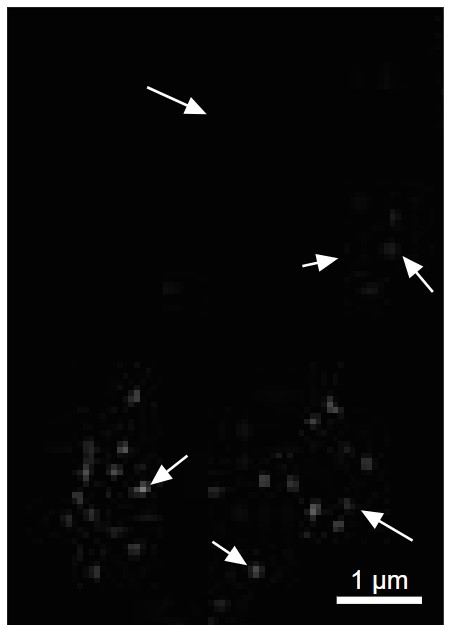
\includegraphics[width=\linewidth]{images/DeepSIM_NMJ_woAO_ROI1_GFP.jpg}
		\caption{GFP:BRP}
		\label{fig:DeepSIM_NMJ_woAO_ROI1_GFP}
	\end{subfigure}
	\begin{subfigure}[t]{0.235\textwidth}
		\centering
		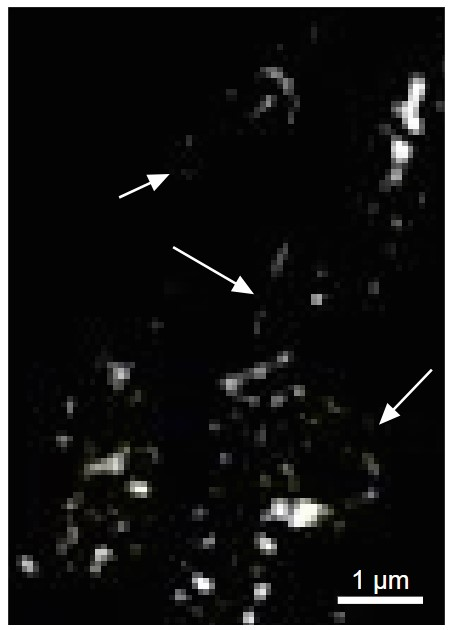
\includegraphics[width=\linewidth]{images/DeepSIM_NMJ_woAO_ROI1_Alexa568.jpg}
		\caption{Alexa568:HRP}
		\label{fig:DeepSIM_NMJ_woAO_ROI1_Alexa568}
	\end{subfigure}
	\begin{subfigure}[t]{0.24\textwidth}
		\centering
		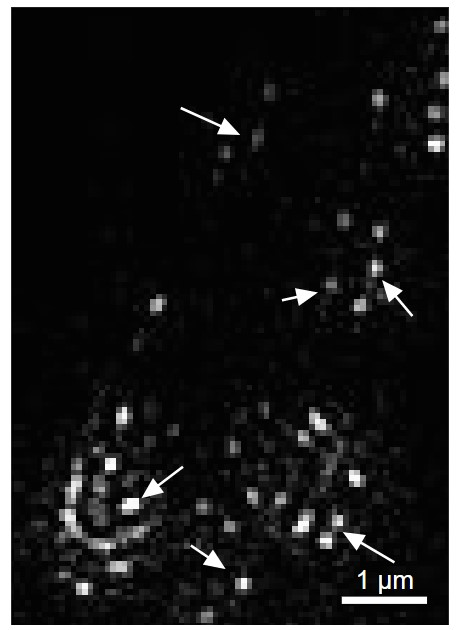
\includegraphics[width=\linewidth]{images/DeepSIM_NMJ_AO_ROI1_GFP.jpg}
		\caption{GFP:BRP}
		\label{fig:DeepSIM_NMJ_AO_ROI1_GFP}
	\end{subfigure}
	\begin{subfigure}[t]{0.242\textwidth}
		\centering
		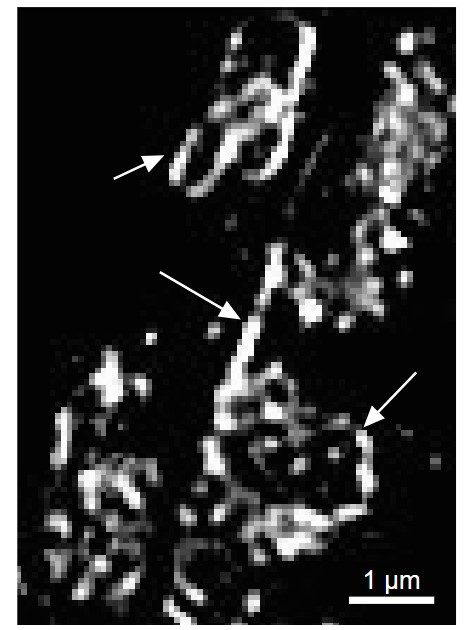
\includegraphics[width=\linewidth]{images/DeepSIM_NMJ_AO_ROI1_Alexa568.jpg}
		\caption{Alexa568:HRP}
		\label{fig:DeepSIM_NMJ_AO_ROI1_Alexa568}
	\end{subfigure}
	
	\hspace{-0.1cm}
	\begin{subfigure}[t]{0.24\textwidth}
		\centering
		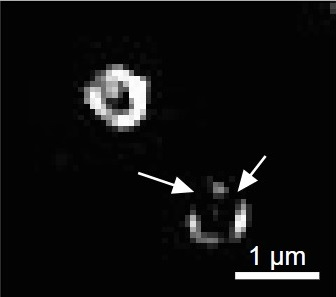
\includegraphics[width=\linewidth]{images/DeepSIM_NMJ_woAO_ROI2_Alexa568.jpg}
		\caption{Alexa568:HRP}
		\label{fig:DeepSIM_NMJ_woAO_ROI2_Alexa568}
	\end{subfigure}
	\hspace{0.05cm}
	\begin{subfigure}[t]{0.24\textwidth}
		\centering
		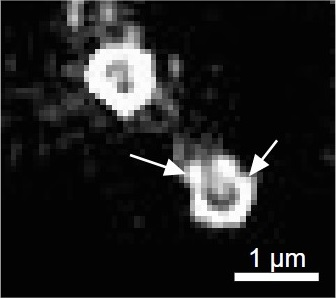
\includegraphics[width=\linewidth]{images/DeepSIM_NMJ_AO_ROI2_Alexa568.jpg}
		\caption{Alexa568:HRP}
		\label{fig:DeepSIM_NMJ_AO_ROI2_Alexa568}
	\end{subfigure}
	\caption[\textit{Drosophila} neuro-muscular junction 
	data acquired on the DeepSIM imaging system]{Maximum intensity 
		projections of 12.75$\mu$m $z$-stacks of neuro-muscular junction 
		samples acquired without (left) and with (right) AO correction. GFP 
		shown in yellow, HRP shown in magenta. The arrows highlight 
		particularly notable areas of improvement where fine details, such as 
		individual puncta, become clearly visible. All images are displayed on the same intensity}
	\label{fig:DeepSIM_NMJ_data}
\end{figure*}

From Equation~\ref{eq:lateral_res_extension_factor_real}, the diffraction 
limited lateral resolution in a SIM reconstruction would be $151$nm and 
$175$nm for the GFP and Alexa568 channels respectively, assuming structures 
of such size exist in the dataset. Figure~\ref{fig:NMJ_ft_data} shows the 
Fourier Transform Lateral (FTL) and Fourier Transform Radial (FTL) of the 
central $z$-slice obtained from the SIMCheck ImageJ 
plug-in\cite{ball2015simcheck}. The red dashed lines in the FTR figures 
show the point where the signal Fourier information is no longer above the 
Fourier noise, which here is used as a proxy for lateral resolution limit 
of the dataset. Without AO correction this is $179$nm and $192$nm for the GFP 
and Alexa568 channels respectively. With AO correction this is $168$nm and 
$188$nm for the GFP and Alexa568 channels respectively. 

Despite the sensorless AO correction being performed on the Alexa568 
channel, only a moderate resolution improvement is observed. Taken 
together with the results from the Argolight slide and the overall contrast 
improvement with AO correction, it is reasonable to conclude that the 
smallest structures in the Alexa568 channel are $\sim165$-$170$nm. A more 
substantial improvement in resolution is observed the GFP channel. The fact 
that both channels benefit from the applied correction despite it being 
acquired from image quality measurements from only one channel implies that 
a significant portion of the aberrations present are achromatic.

\begin{figure*}
	\vspace{-1cm}
	\begin{subfigure}[t]{0.45\textwidth}
		\centering
		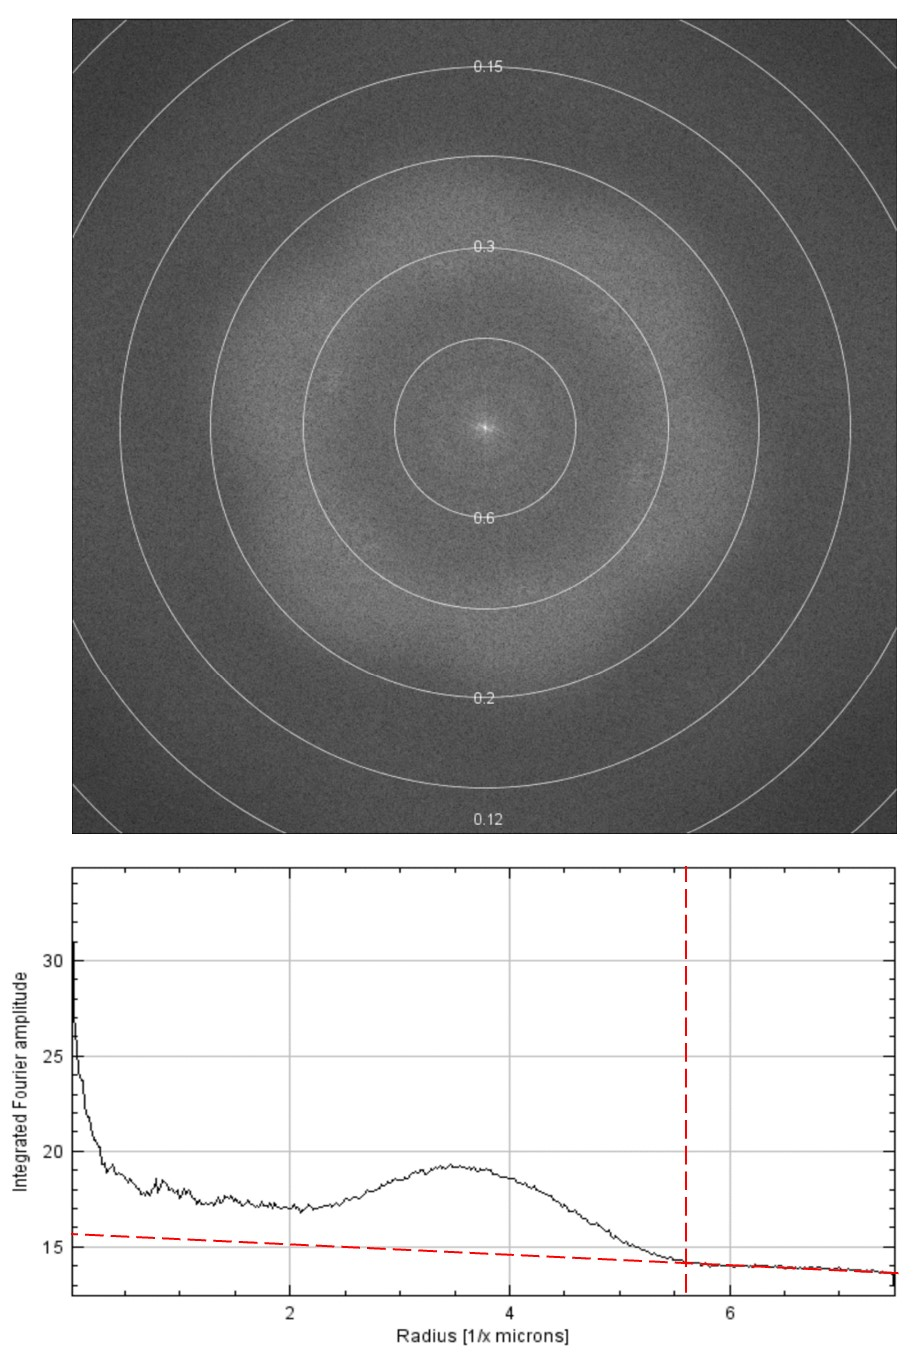
\includegraphics[width=\linewidth]{images/DeepSIM_NMJ_woAO_GFP_ft_and_plot.jpg}
		\caption{Without AO, GFP channel}
		\label{fig:DeepSIM_NMJ_woAO_GFP_ft_and_plot}
	\end{subfigure}
	\begin{subfigure}[t]{0.45\textwidth}
		\centering
		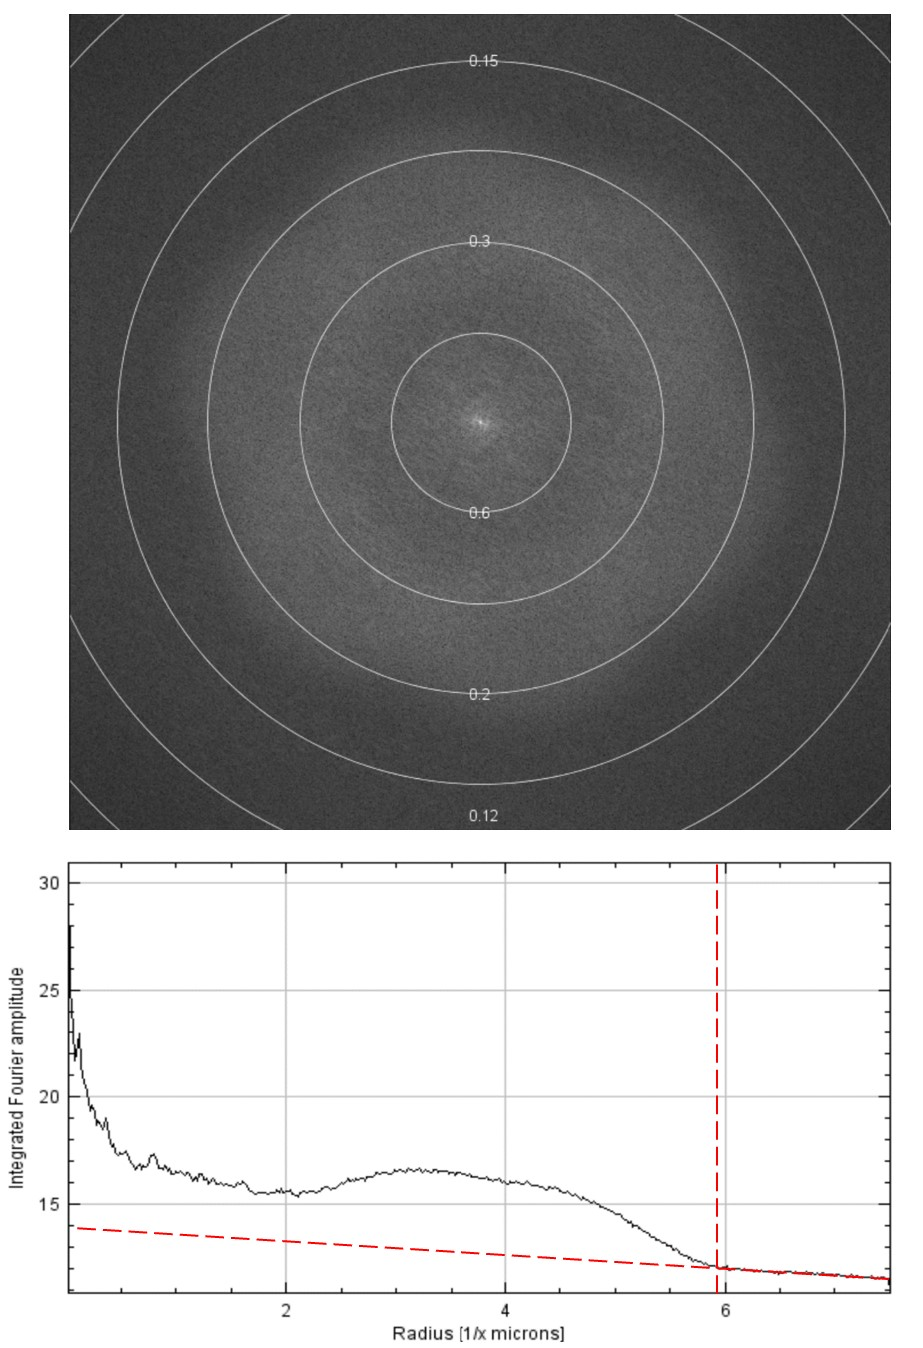
\includegraphics[width=\linewidth]{images/DeepSIM_NMJ_AO_GFP_ft_and_plot.jpg}
		\caption{With AO, GFP channel}
		\label{fig:DeepSIM_NMJ_AO_GFP_ft_and_plot}
	\end{subfigure}
	
	
	\begin{subfigure}[t]{0.45\textwidth}
		\centering
		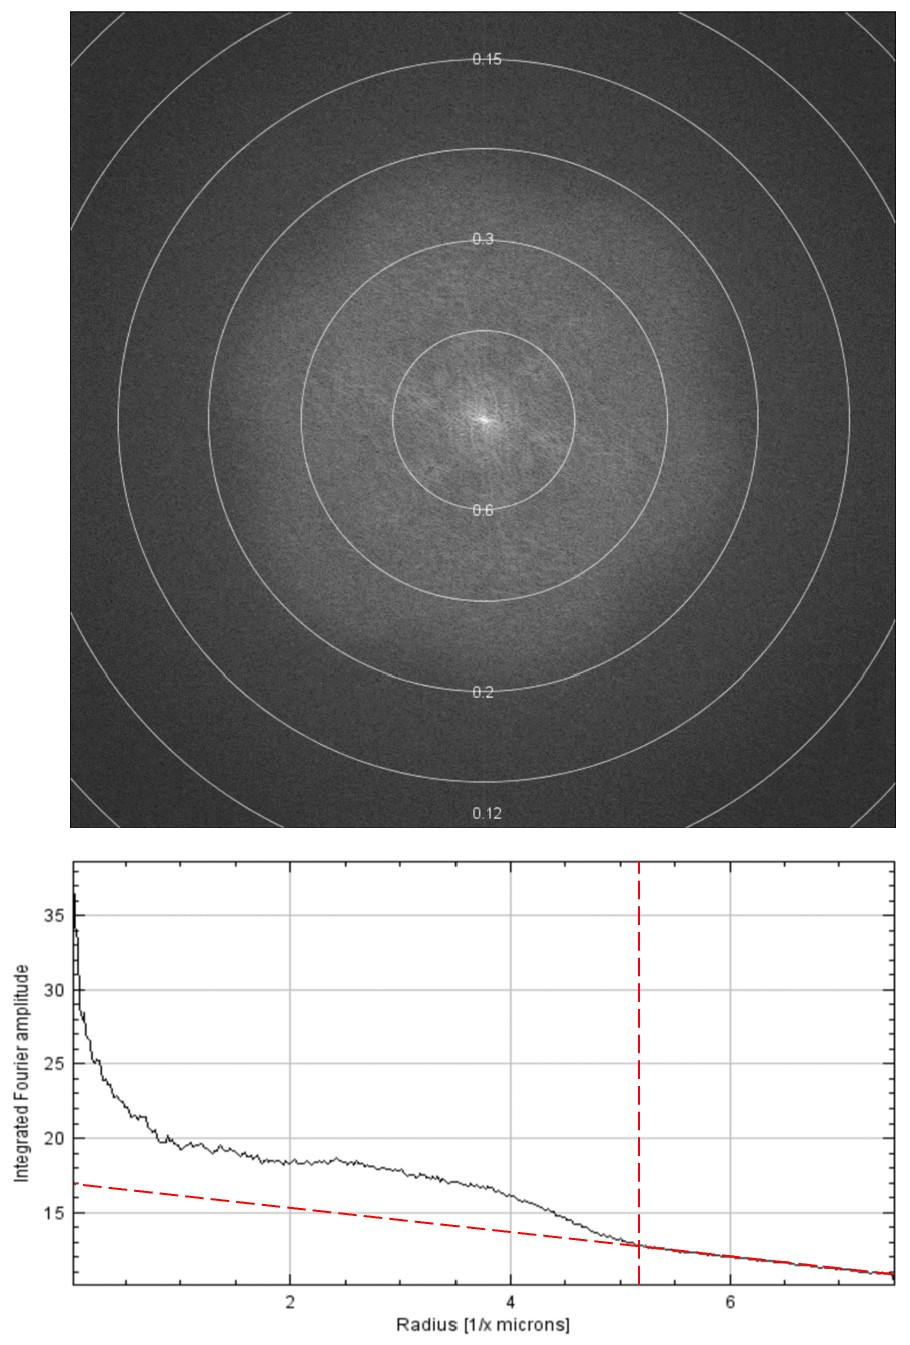
\includegraphics[width=\linewidth]{images/DeepSIM_NMJ_woAO_Alexa568_ft_and_plot.jpg}
		\caption{Without AO, Alexa568 channel}
		\label{fig:DeepSIM_NMJ_woAO_Alexa568_ft_and_plot}
	\end{subfigure}
	\begin{subfigure}[t]{0.45\textwidth}
		\centering
		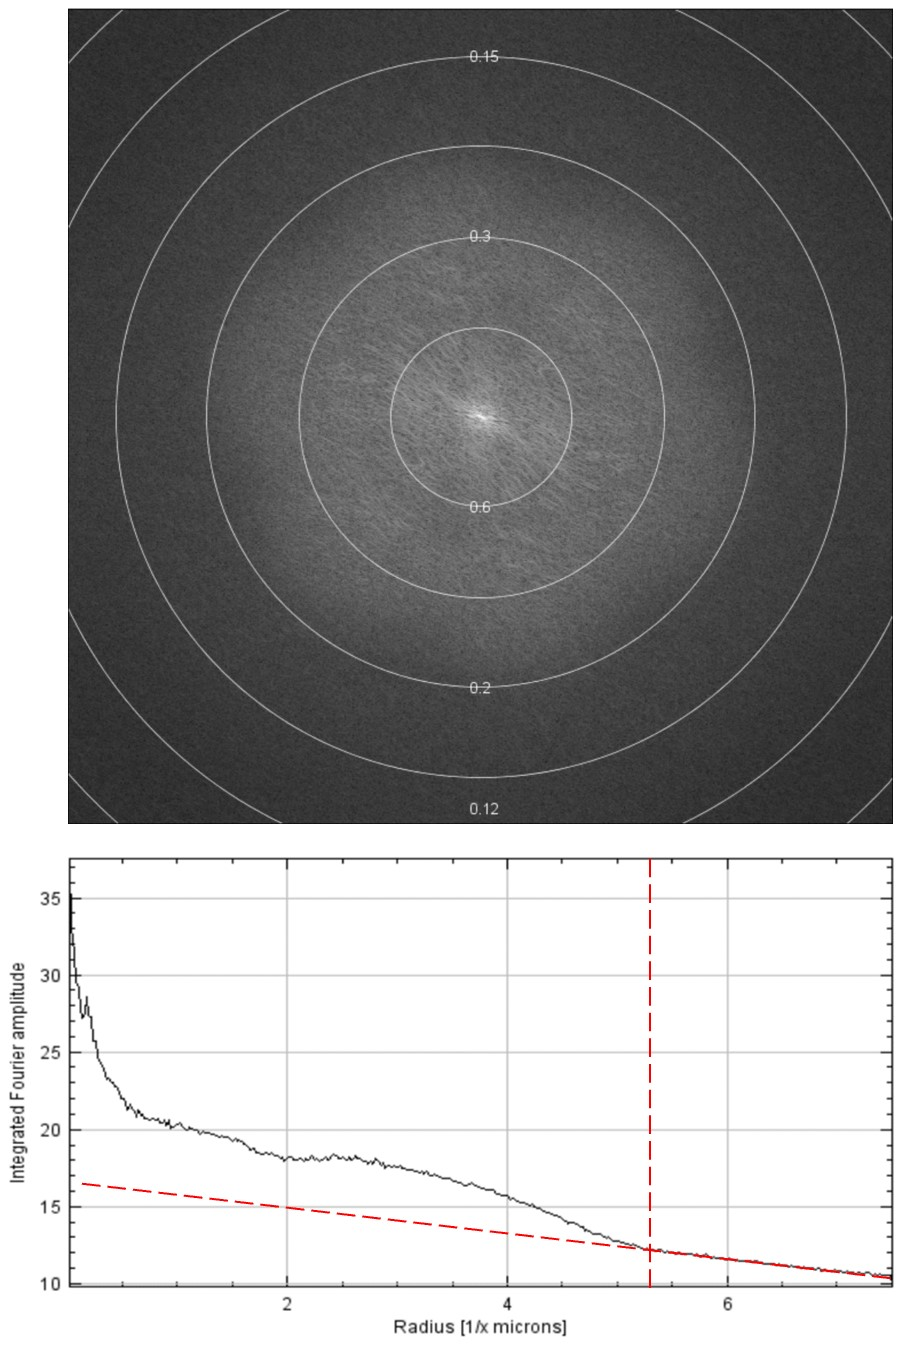
\includegraphics[width=\linewidth]{images/DeepSIM_NMJ_AO_Alexa568_ft_and_plot.jpg}
		\caption{With AO, Alexa568 channel}
		\label{fig:DeepSIM_NMJ_AO_Alexa568_ft_and_plot}
	\end{subfigure}
	\caption[Fourier plots of \textit{Drosophila} neuro-muscular junction 
	data acquired on the DeepSIM imaging system]{Fourier plots of 
		\textit{Drosophila} neuro-muscular junction data acquired on the 
		DeepSIM imaging system. Each subplot shows the Fourier Transform 
		Lateral (FTL) (top) and Fourier	Transform Radial (FTR) (bottom) of the 
		central $z$-slice from the SIMCheck ImageJ 
		plug-in\cite{ball2015simcheck} for \textbf{(a)} GFP channel without AO 
		correction \textbf{(b)} Alexa568 channel without AO correction 
		\textbf{(c)} GFP channel with AO correction \textbf{(d)} Alexa568 
		channel with AO correction}
	\label{fig:NMJ_ft_data}
\end{figure*}
